\section{Introduction}\label{sec:intro}

The PSBLAS library, developed with the aim to facilitate the
parallelization of computationally intensive scientific applications,
is designed to address parallel implementation of iterative solvers
for sparse linear systems through the distributed memory paradigm.  It
includes routines for multiplying sparse matrices by dense matrices,
solving block diagonal systems with triangular diagonal entries,
preprocessing sparse matrices, and contains additional routines for
dense matrix operations.  The current implementation of PSBLAS
addresses a distributed memory execution model operating with message
passing. 

The PSBLAS library version 3 is  implemented in
 the Fortran~2003~\cite{metcalf} programming language, with reuse and/or
 adaptation of  existing Fortran~77 and Fortran~95 software, plus a
 handful of C  routines. 

The use of Fortran~2003 offers a number of advantages over Fortran~95,
mostly in the handling of requirements for evolution and adaptation of
the library to new computing architectures and integration of
new algorithms. 
For a detailed discussion of our design see~\cite{Sparse03}; other
works discussing advanced programming in Fortran~2003
include~\cite{DesPat:11,RouXiaXu:11}; sufficient support for
Fortran~2003 is now available from many compilers, including the GNU
Fortran compiler from the Free Software Foundation (as of version 4.8). 


Previous approaches have been based on mixing Fortran~95, with its
support for object-based design, with other languages; these have
been advocated by a number of authors, 
e.g.~\cite{machiels}.  Moreover, the Fortran~95 facilities for dynamic
memory management and interface overloading greatly enhance the
usability of the PSBLAS 
subroutines. In this way, the library can take care of runtime memory
requirements that are quite difficult or even impossible to predict at
implementation or compilation time.  

The presentation of the
PSBLAS library follows the general structure of the proposal for
serial Sparse BLAS~\cite{sblas97,sblas02}, which in its turn is based on the
proposal for BLAS on dense matrices~\cite{BLAS1,BLAS2,BLAS3}.

The applicability of sparse iterative solvers to many different areas
causes some terminology problems because the same concept may be
denoted through different names depending on the application area. The
PSBLAS features presented in this document will be discussed referring
to a   finite difference discretization of a Partial Differential
Equation (PDE). However, the scope of the library is wider than
that: for example, it can be applied to finite element discretizations
of PDEs, and even to different classes of problems such as nonlinear
optimization, for example in optimal control problems.

The design of a solver for sparse linear systems is driven by many
conflicting objectives, such as limiting occupation of storage
resources, exploiting regularities in the input data, exploiting
hardware characteristics of the parallel platform.  To achieve an
optimal communication to computation ratio on distributed memory
machines it is essential to keep the {\em data locality} as high as
possible; this can be done through an appropriate data allocation
strategy.  The choice of the preconditioner is another very important
factor that affects efficiency of the implemented application. Optimal
data distribution requirements for a given preconditioner may conflict
with distribution requirements of the rest of the solver. Finding the
optimal trade-off may be very difficult because it is application
dependent.  Possible solutions to these problems and other important
inputs to the development of the PSBLAS software package have come from
an established experience in applying the PSBLAS solvers to
computational fluid dynamics applications.

\section{General overview}
\label{sec:overview} 
The PSBLAS library is designed to handle the implementation of
iterative solvers for sparse linear systems on distributed memory
parallel computers.  The system coefficient matrix $A$ must be square;
it may be real or complex, nonsymmetric, and its sparsity pattern
needs not to be symmetric.  The serial computation parts are based on
the serial sparse BLAS, so that any extension made to the data
structures of the serial kernels is available to the parallel
version. The overall design and parallelization strategy have been
influenced by the structure of the ScaLAPACK parallel
library.  The layered structure of the PSBLAS library
is shown in figure~\ref{fig:psblas}; lower layers of the library
indicate an encapsulation relationship with upper layers. The ongoing
discussion focuses on the Fortran~2003 layer immediately below the
application layer.
The serial parts of the computation on each process are executed through
calls to the serial sparse BLAS subroutines. 
In a similar way, the inter-process message exchanges are encapsulated
in an applicaiton layer that has been strongly inspired by the  Basic
Linear Algebra Communication Subroutines (BLACS) library~\cite{BLACS}.  
Usually  there is no need to deal directly with MPI;  however, in some
cases, MPI routines are used directly to improve efficiency. For
further details on our communication layer see Sec.~\ref{sec:parenv}.
%% We assume that the user program has initialized a BLACS process grid
%% with one column and as many rows as there are processes; the PSBLAS
%% initialization routines will take the communication context for this
%% grid and store internally for further use. 

\begin{figure}[h] 
\begin{center}
\ifcase\pdfoutput
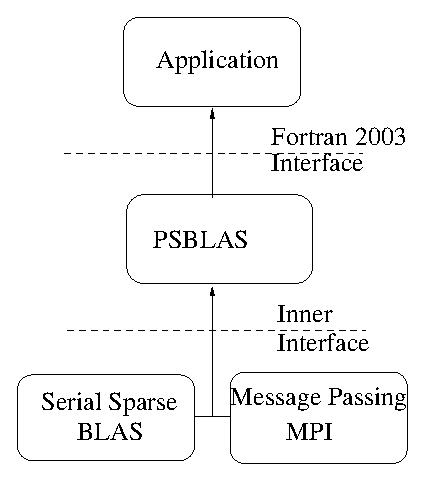
\includegraphics[scale=0.65]{figures/psblas.eps}
\or
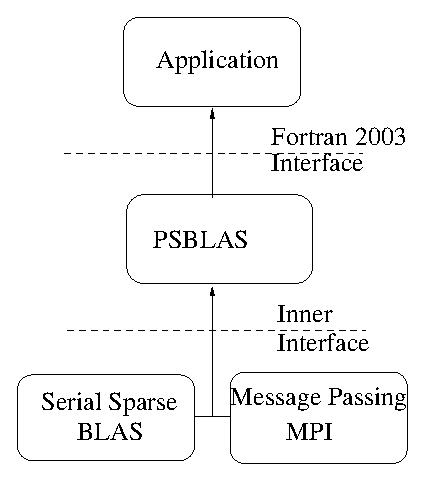
\includegraphics[scale=0.65]{figures/psblas}
\fi
\end{center}
\caption{PSBLAS library components hierarchy.\label{fig:psblas}}
\end{figure}


The type of linear system matrices that we address  typically arise in the
numerical solution of PDEs;  in such a context,
it is necessary to pay special attention to the
structure of the problem from which the application originates. 
The nonzero pattern of a matrix arising from the
discretization of a PDE is influenced by various factors, such as the
shape of the  domain, the discretization strategy, and
the equation/unknown ordering. The matrix itself can be interpreted as
the  adjacency matrix of the graph associated with the discretization
mesh. 

The distribution of the coefficient matrix for the linear system is
based on the ``owner computes'' rule: 
the variable associated to each mesh point is assigned to a process
that will  own the corresponding row in the coefficient matrix and
will  carry out all related computations. This allocation strategy 
is equivalent to a partition of the discretization mesh into {\em
sub-domains}. 
Our library  supports any distribution that keeps together 
the coefficients of each matrix row; there are no other constraints on
the variable assignment. 
This choice is consistent with simple  data distributions 
%commonly used in ScaLAPACK 
such as  \verb|CYCLIC(N)| and \verb|BLOCK|, 
as well as completely arbitrary assignments of
equation indices to processes. 
In particular it is consistent with the
usage of graph partitioning tools commonly available in the
literature, e.g. METIS~\cite{METIS}.
Dense vectors  conform  to sparse
matrices, that is, the entries of a vector follow the same distribution
of the matrix rows.  

We assume that the sparse matrix is built in parallel, where each
process generates its own portion. We never require that the entire
matrix be available on a single node. However, it is possible
to hold the entire matrix in one process and distribute it
explicitly\footnote{In our prototype implementation  we provide 
sample scatter/gather routines.}, even though  the resulting memory 
bottleneck would make this option unattractive in most  cases. 


\subsection{Basic Nomenclature}


Our computational model implies that the data allocation on the
parallel distributed memory machine is guided by the structure of the
physical model, and specifically by the discretization mesh of the
PDE. 

Each point of the discretization mesh will have (at least) one
associated equation/variable, and therefore one index. We say that
point  $i$ {\em depends\/} on point $j$ if the  equation for a
variable associated with $i$ contains a term in $j$,  or equivalently
if $a_{ij} \ne0$.  
After the partition of the discretization mesh into {\em sub-domains\/}
assigned to the parallel processes,
we classify the  points of a given sub-domain as following.
\begin{description}
\item[Internal.] An internal point of
 a given domain {\em depends} only on  points of the
same domain. 
If all points of a domain are assigned to one
process, then a computational step (e.g., a
matrix-vector product) of the 
equations associated with the internal points  requires no data
items from other domains and no communications.

\item[Boundary.] A point of
a given domain is a boundary point if it {\em depends} on  points
belonging to other domains.

\item[Halo.] A halo point for a given domain is a point belonging to
another domain such that there is a boundary point which {\em depends\/}
on it. Whenever performing a computational step, such as a
matrix-vector product, the values associated with halo points are
requested from other domains. A boundary point of a given 
domain is usually a halo point for some other domain\footnote{This is
  the normal situation when the pattern of the sparse matrix is
  symmetric, which is equivalent to say that the interaction between
  two variables is reciprocal. If the matrix pattern is non-symmetric
  we may have one-way interactions, and these could cause a situation
  in which a boundary point is not a halo point for its neighbour.}; therefore
the cardinality of the boundary points set denotes the amount of data
 sent to other domains. 
\item[Overlap.] An overlap point is a boundary point assigned to
multiple domains. Any operation that involves an overlap point
has to be replicated for each assignment. 
\end{description}
Overlap points do not usually exist in the basic data
distributions; however they are a feature of Domain Decomposition
Schwarz preconditioners which are the subject of related research
work~\cite{2007c,2007d}.

We denote the sets of  internal, boundary and halo points for a given
subdomain  by $\cal I$, $\cal B$ and $\cal H$.
Each subdomain is assigned to one process; each process usually
owns one subdomain, although the user may choose to assign more than
one subdomain to a process.  If each process $i$ owns one
subdomain, the number of rows in the local sparse matrix is
$|{\cal I}_i| + |{\cal B}_i|$, and the number of local columns
(i.e. those for which there exists at least one non-zero entry in the
local rows)  is $|{\cal I}_i| + |{\cal B}_i| +|{\cal H}_i|$.

\begin{figure}[h] 
\begin{center}
\ifcase\pdfoutput
%\rotatebox{-90}{
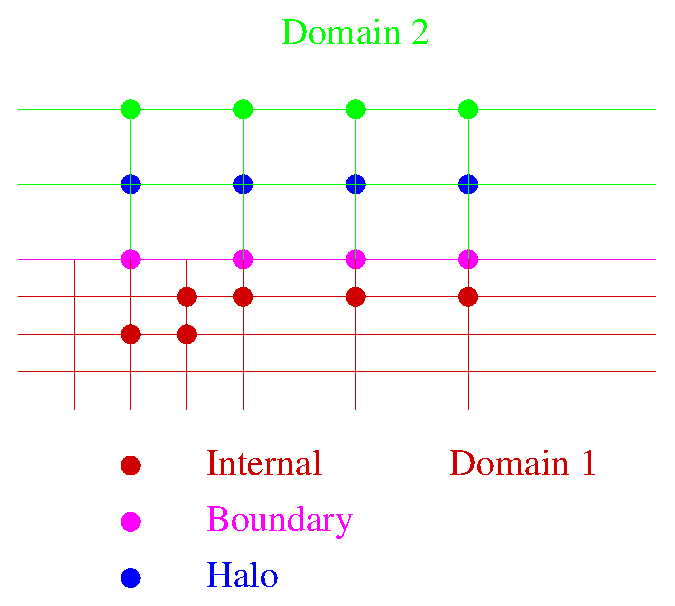
\includegraphics[scale=0.65]{figures/points.eps}%}
\or
\rotatebox{-90}{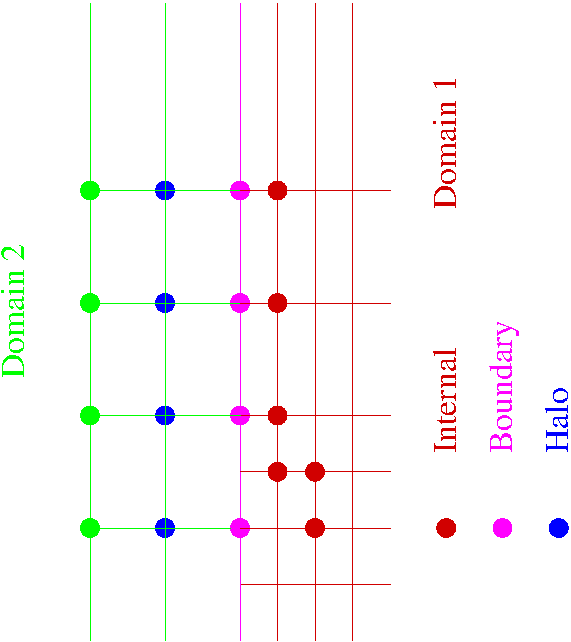
\includegraphics[scale=0.65]{figures/points}}
\fi
\end{center}
\caption{Point classfication.\label{fig:points}}
\end{figure}

This classification of mesh points guides the naming scheme that we
adopted in the library internals and in the data structures. We
explicitly note that ``Halo'' points are also often called ``ghost''
points in the literature. 



\subsection{Library contents}

The PSBLAS library consists of various classes of subroutines:
\begin{description}
\item[Computational routines] comprising:
\begin{itemize}
\item Sparse matrix by dense matrix product; 
\item Sparse triangular
systems solution for block diagonal matrices;
\item Vector and matrix norms;
\item Dense matrix sums;
\item Dot products.
\end{itemize} 
\item[Communication routines] handling halo and overlap
  communications;
\item[Data management and auxiliary routines] including:
\begin{itemize}
\item Parallel environment management
\item Communication descriptors allocation;
\item Dense and sparse matrix allocation;
\item Dense and sparse matrix build and update;
\item Sparse matrix and data distribution preprocessing.
\end{itemize} 
\item[Preconditioner routines]
\item[Iterative methods] a subset of Krylov subspace iterative
  methods
\end{description}
The following naming scheme has been adopted for all the symbols
internally defined in the PSBLAS software package:
\begin{itemize}
\item all symbols (i.e. subroutine names, data types...) are
  prefixed by \verb|psb_| 
\item all data type names are suffixed by \verb|_type|
\item all constants are suffixed by \verb|_|
\item all top-level subroutine names follow the rule \verb|psb_xxname| where
  \verb|xx| can be either:
  \begin{itemize}
  \item \verb|ge|: the routine is related to dense data, 
  \item \verb|sp|: the routine is related to sparse data, 
  \item \verb|cd|: the routine is related to communication descriptor
        (see~\ref{sec:datastruct}).
  \end{itemize}
  For example the \verb|psb_geins|, \verb|psb_spins| and
  \verb|psb_cdins| perform the same action (see~\ref{sec:toolsrout}) on
  dense matrices, sparse matrices and communication descriptors
  respectively.
  Interface overloading allows the usage of the same subroutine
  names  for both real and complex data.
\end{itemize}
In the description of the subroutines, arguments or argument entries
are classified as:
\begin{description}
\item[global] For input arguments, the value must be the same on all processes
  participating in the subroutine call; for output arguments the value
  is guaranteed to be the same.
\item[local] Each process has its own value(s) independently.
\end{description}
To finish our general description, we define a version string with the
constant 
\[ \verb|psb_version_string_|\]
whose current value is \verb|3.4.0|

\subsection{Application structure}
\label{sec:appstruct}

The main underlying principle of the PSBLAS library is that the
library objects are created and exist with reference to a discretized
space to which there corresponds an index space and a matrix sparsity
pattern. As an example, consider a cell-centered finite-volume
discretization of  the Navier-Stokes equations on a simulation domain;
the index space $1\dots n$ is isomorphic to the set of cell centers,
whereas the pattern of the associated linear system matrix is
isomorphic to the adjacency graph imposed on the discretization mesh
by the discretization stencil. 

Thus the first order of business is to establish an index space, and
this is done with a call to  \verb|psb_cdall| in which we specify the
size of the index space $n$ and the allocation of the elements of the
index space to the various processes making up the MPI (virtual)
parallel machine. 

The index space is partitioned among processes, and this creates a
mapping from the ``global'' numbering $1\dots n$ to a numbering
``local'' to each process; each process $i$ will own a certain subset
$1\dots n_{\hbox{row}_i}$, each element of which corresponds to a certain
element of $1\dots n$. The user does not set explicitly this mapping;
when the application needs to indicate to which element of the index
space a certain item is related, such as the row and column index of a
matrix coefficient, it does so in the ``global'' numbering, and the
library will translate into the appropriate ``local'' numbering. 

For  a given index space $1\dots n$ there are many possible associated
topologies, i.e. many different discretization stencils; thus the
description of the index space is not completed until the user has
defined a sparsity pattern, either explicitly through \verb|psb_cdins|
or implicitly through \verb|psb_spins|. The descriptor is finalized
with a call to \verb|psb_cdasb| and a sparse matrix with a call to
\verb|psb_spasb|. After \verb|psb_cdasb| each process $i$ will have
defined a set of ``halo'' (or ``ghost'') indices
$n_{\hbox{row}_i}+1\dots n_{\hbox{col}_i}$, denoting elements of the index
space that are \emph{not} assigned to process $i$; however the
variables associated with them are needed to complete computations
associated with the sparse matrix $A$, and thus they have to be
fetched from (neighbouring) processes. The descriptor of the index
space is built exactly for the purpose of properly sequencing the
communication steps required to achieve this objective. 

A simple application structure will walk through the index space
allocation, matrix/vector creation and linear system solution as
follows:
\begin{enumerate}
\item Initialize parallel environment with \verb|psb_init|
\item Initialize index space with \verb|psb_cdall|
\item Allocate sparse matrix and dense vectors with \verb|psb_spall|
  and \verb|psb_geall|
\item Loop over all local rows, generate matrix and vector entries,
  and insert them with \verb|psb_spins| and \verb|psb_geins|
\item Assemble the various entities: 
\begin{enumerate}
\item \verb|psb_cdasb|
\item \verb|psb_spasb|
\item \verb|psb_geasb|
\end{enumerate}
\item Choose the preconditioner to be used with \verb|prec%init| and
  build it with \verb|prec%build|\footnote{The subroutine style {\tt
      psb\_precinit} and {\tt psb\_precbl} are still supported for
    backward compatibility}. 
\item Call the iterative method of choice, e.g. \verb|psb_bicgstab|
\end{enumerate}
This is the structure of the sample programs in the directory 
\verb|test/pargen/|. 

For a simulation in which the same discretization mesh is used over
multiple time steps, the following structure may be more appropriate:
\begin{enumerate}
\item Initialize parallel environment with \verb|psb_init|
\item Initialize index space with \verb|psb_cdall|
\item Loop over the topology of the discretization mesh and build the
  descriptor with \verb|psb_cdins|
\item Assemble the descriptor with \verb|psb_cdasb|
\item Allocate the sparse matrices and dense vectors with
  \verb|psb_spall| and \verb|psb_geall|
\item Loop over the time steps: 
\begin{enumerate}
\item If after first time step, 
  reinitialize the sparse matrix with \verb|psb_sprn|; also zero out
  the dense vectors;
\item Loop over the mesh, generate the coefficients and insert/update
  them with \verb|psb_spins| and \verb|psb_geins|
\item Assemble with \verb|psb_spasb| and \verb|psb_geasb|
\item Choose and build preconditioner with \verb|prec%init| and
  \verb|prec%build|
\item Call the iterative method of choice, e.g. \verb|psb_bicgstab|
 \end{enumerate}
\end{enumerate}
The insertion routines will be called as many times as needed; 
they only need to  be called on the data that is actually
allocated to the current process, i.e. each process generates its own
data. 

In principle there is no specific order in the calls to
\verb|psb_spins|, nor is there a requirement to build a matrix row in
its entirety before calling the routine; this allows the application
programmer to walk through the discretization mesh element by element,
generating the main part of a given matrix row but also contributions
to the rows corresponding to neighbouring elements. 

From a functional point of view it is even possible to execute one
call for each nonzero coefficient; however this would have a
substantial computational overhead. It is therefore advisable to pack
a certain amount of data into each call to the insertion routine, say
touching on a few tens of rows; the best performng value would depend
on both the architecture of the computer being used and on the problem
structure. 
At the opposite extreme, it would be possible to generate the entire
part of a coefficient matrix residing on a process and pass it in a
single call to \verb|psb_spins|; this, however, would entail a
doubling of memory occupation, and thus would be almost always far
from optimal. 

\subsubsection{User-defined index mappings}
\label{sec:usermaps}
PSBLAS supports user-defined global to local index mappings, subject
to the constraints outlined in sec.~\ref{sec:appstruct}: 
\begin{enumerate}
\item The set of indices owned locally must be mapped to the set
  $1\dots n_{\hbox{row}_i}$;
\item The set of halo points must be mapped to the set
  $n_{\hbox{row}_i}+1\dots n_{\hbox{col}_i}$;
\end{enumerate}
but otherwise the mapping is arbitrary. The user application is
responsible to ensure consistency of this mapping; some errors may be
caught by the library, but this is not guaranteed. 
The application structure to
support this usage is as follows:
\begin{enumerate}
\item Initialize index space with
  \verb|psb_cdall(ictx,desc,info,vl=vl,lidx=lidx)| passing the vectors 
  \verb|vl(:)| containing the set of global indices owned by the
  current process and   \verb|lidx(:)| containing the corresponding
  local indices;
\item Add the halo points \verb|ja(:)| and their associated local
  indices \verb|lidx(:)|  with a(some) call(s) to
  \verb|psb_cdins(nz,ja,desc,info,lidx=lidx)|; 
\item Assemble the descriptor with \verb|psb_cdasb|;
\item Build the sparse matrices and vectors, optionally making use in
  \verb|psb_spins| and \verb|psb_geins| of the \verb|local| argument
  specifying that the indices in \verb|ia|, \verb|ja| and \verb|irw|,
  respectively, are already local indices. 
\end{enumerate}


\subsection{Programming model}

The PSBLAS librarary is based on the Single Program Multiple Data
(SPMD) programming model: each process participating in the
computation performs the same actions on a chunk of data. Parallelism
is thus data-driven. 

Because of this structure, many subroutines coordinate their action
across the various processes, thus providing an implicit
synchronization point, and therefore \emph{must} be
called simultaneously by all processes participating in the
computation. This is certainly true for the data allocation and
assembly routines, for  all the computational routines and for some of
the tools routines.

However there are many cases where no synchronization, and indeed no
communication among processes, is implied; for instance, all the routines in
sec.~\ref{sec:datastruct} are only acting on the local data structures,
and thus may be called independently. The most important case is that
of the coefficient insertion routines: since the number of
coefficients in the sparse and dense matrices varies among the
processors, and since the user is free to choose an arbitrary order in
builiding the matrix entries, these routines cannot imply a
synchronization. 

Throughout this user's guide each subroutine will be clearly indicated
as:
\begin{description}
\item[Synchronous:] must be called simultaneously by all the
  processes in the relevant communication context;
\item[Asynchronous:] may be called in a totally independent manner.
\end{description}

%%% Local Variables: 
%%% mode: latex
%%% TeX-master: "userguide"
%%% End: 
